\newchapt{Boundary Vectorization}{chapt5}{Boundary Vectorization}

After the keyslices are detected, $N_K$ keyslices will be identified
from a total of $N_A$ image slices.
Depending on the threshold $\tau_{d}$, $N_K$ is usually about one to two
orders of magnitude smaller than $N_A$, e.g., $N_K/N_A$ is 0.06 when
$\tau_d$ = 4.0 for the example in \Figb{IR_2_DXF}.
To generate the 3D model, these keyslice images need to be vectorized to
represent the contours of the building facade.
The difficulty of the problem lies in outliers and holes of non-perfect images.
We proposed a general framework based on an adaptive 2D ball-pivot algorithm (BPA) 
 to efficiently suppress the noisy, fill holes and generate contours for those images.

\section{Ball Pivot Algorithm (BPA)}
\label{sec:BPA}

STARTING POINT SELECTION
\\
\\
GAP DETECTION
\\
\\
RIGHT ANGLE RESHAPE
\\
\\


There exists numerous works on boundary vectorization,
such as those described in \cite{DP_RP,DP_LC,DP_AAKMT}.
However, these approaches
only consider the cases where perfect raster image data is provided.
For non-perfect data, these proposed methods were failed in various cases.
The problem considered here is to compute contours
for non-perfect binary images which may contain holes
along the boundary as well as noise or outliers
inside the boundary. Here, {\it boundary} refers to the
out-most region of any raster image and
{\it contour} refers to a vectorized boundary.


The Douglas-Peucker (DP) algorithm \cite{DP_DP} is widely used
to compute boundary vectorization for binary images.
Although  with the improvement of implementation described in \cite{DP_HS, DP_HS94},
the complexity of this approach is of $O(nlogn)$, this method cannot fill the
holes of the noisy data or handle the case
where spurious interior points are presented.
Agarwal et al. \cite{DP_AV} considered the problem of
approximating a polygon chain using another one to minimize the number of
vertices. However, for a raster image, the vertices
defining the contour were not known.
For example, \Figa{failed_case} shows a binary cross-section
image of a 3D point cloud data of a building. \Figb{failed_case} shows
the contour generated from DP algorithm. The problem is that there are
a lot of holes along the contour and the noise data inside of the
boundary are modeled inappropriately.
To tackle these issues, a general boundary vectorization framework is proposed
based on ball-pivoting algorithm (BPA) \cite{BPA_BMRS} which was used
originally on 3D point cloud data process to generate 3D mesh representation.
\Figc{failed_case} shows
the contour computed by the proposed framework which fills holes between gaps
and suppresses noise inside the boundary.


\begin{figure*}[hbtp]
\begin{center}
\begin{tabular}{c}
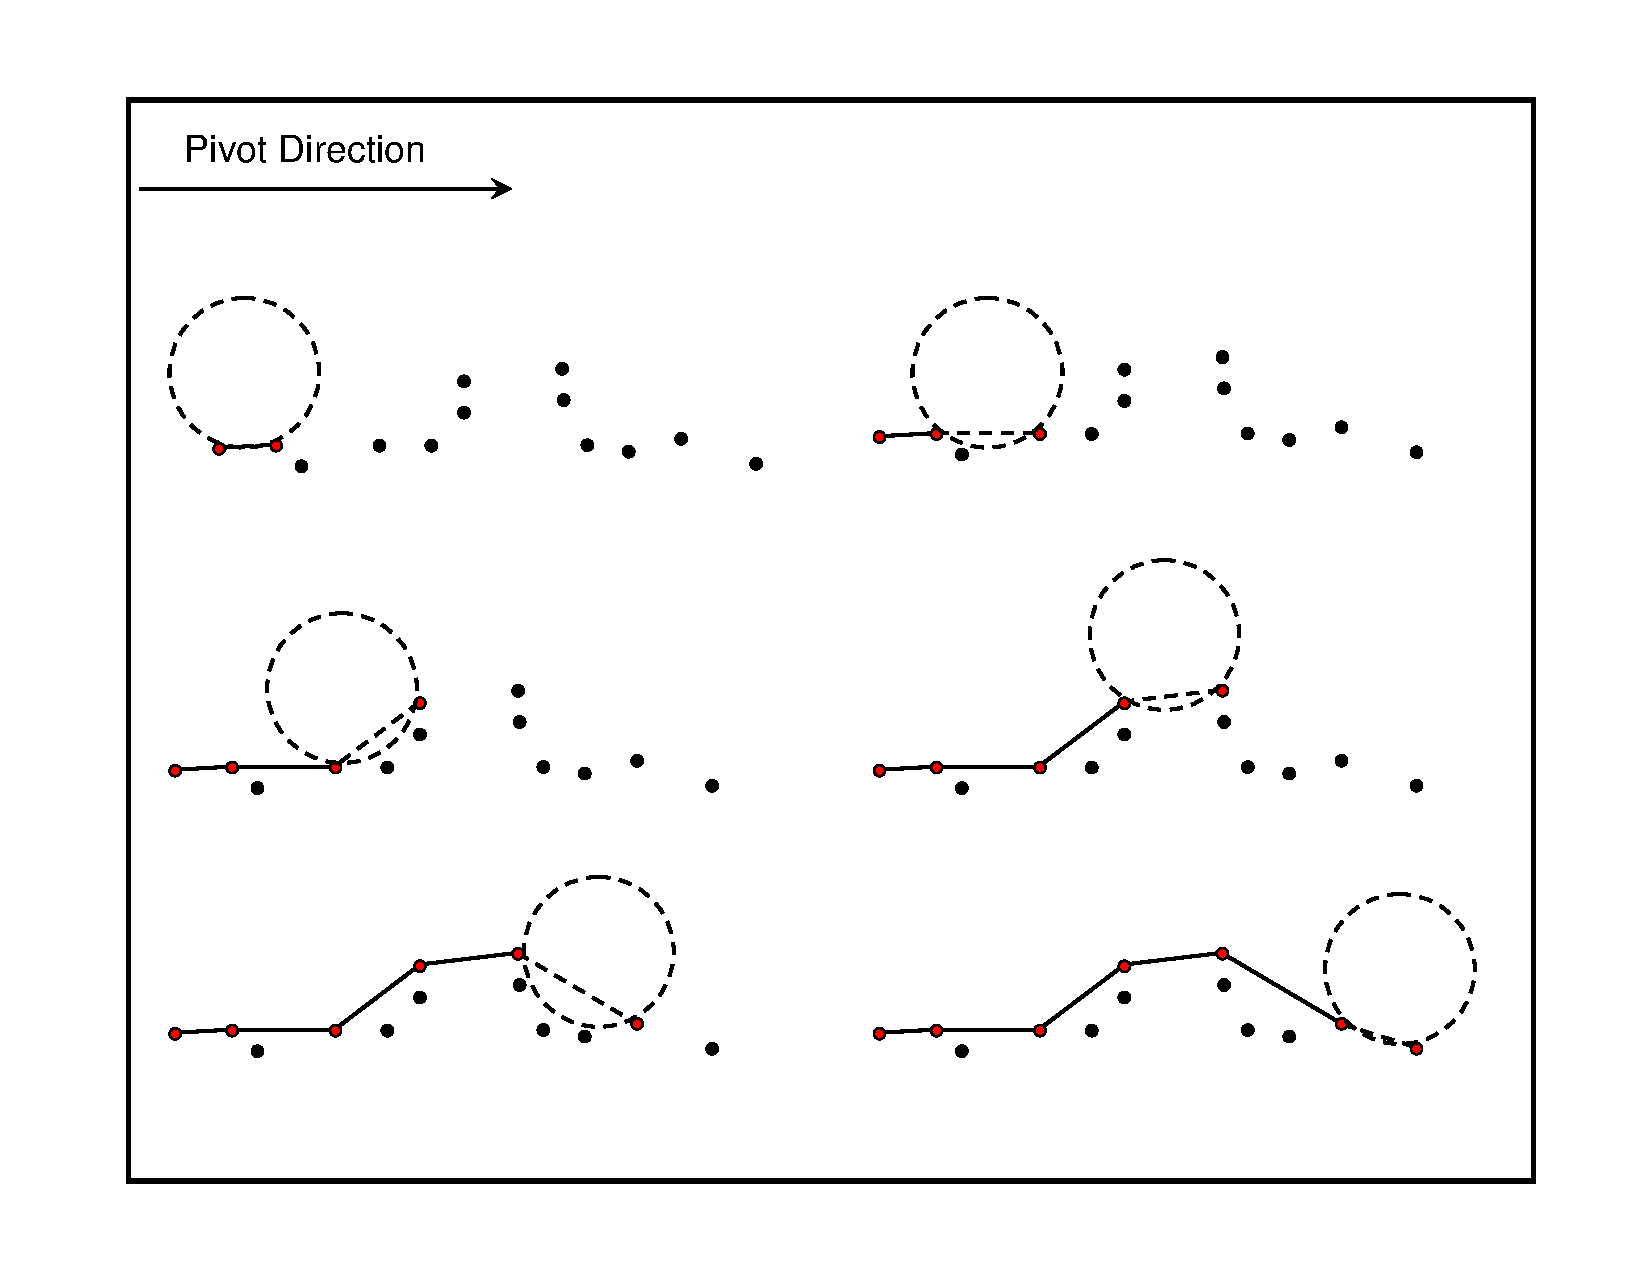
\includegraphics[width=0.8\textwidth]{BPA_init.pdf} \\
(a) \\
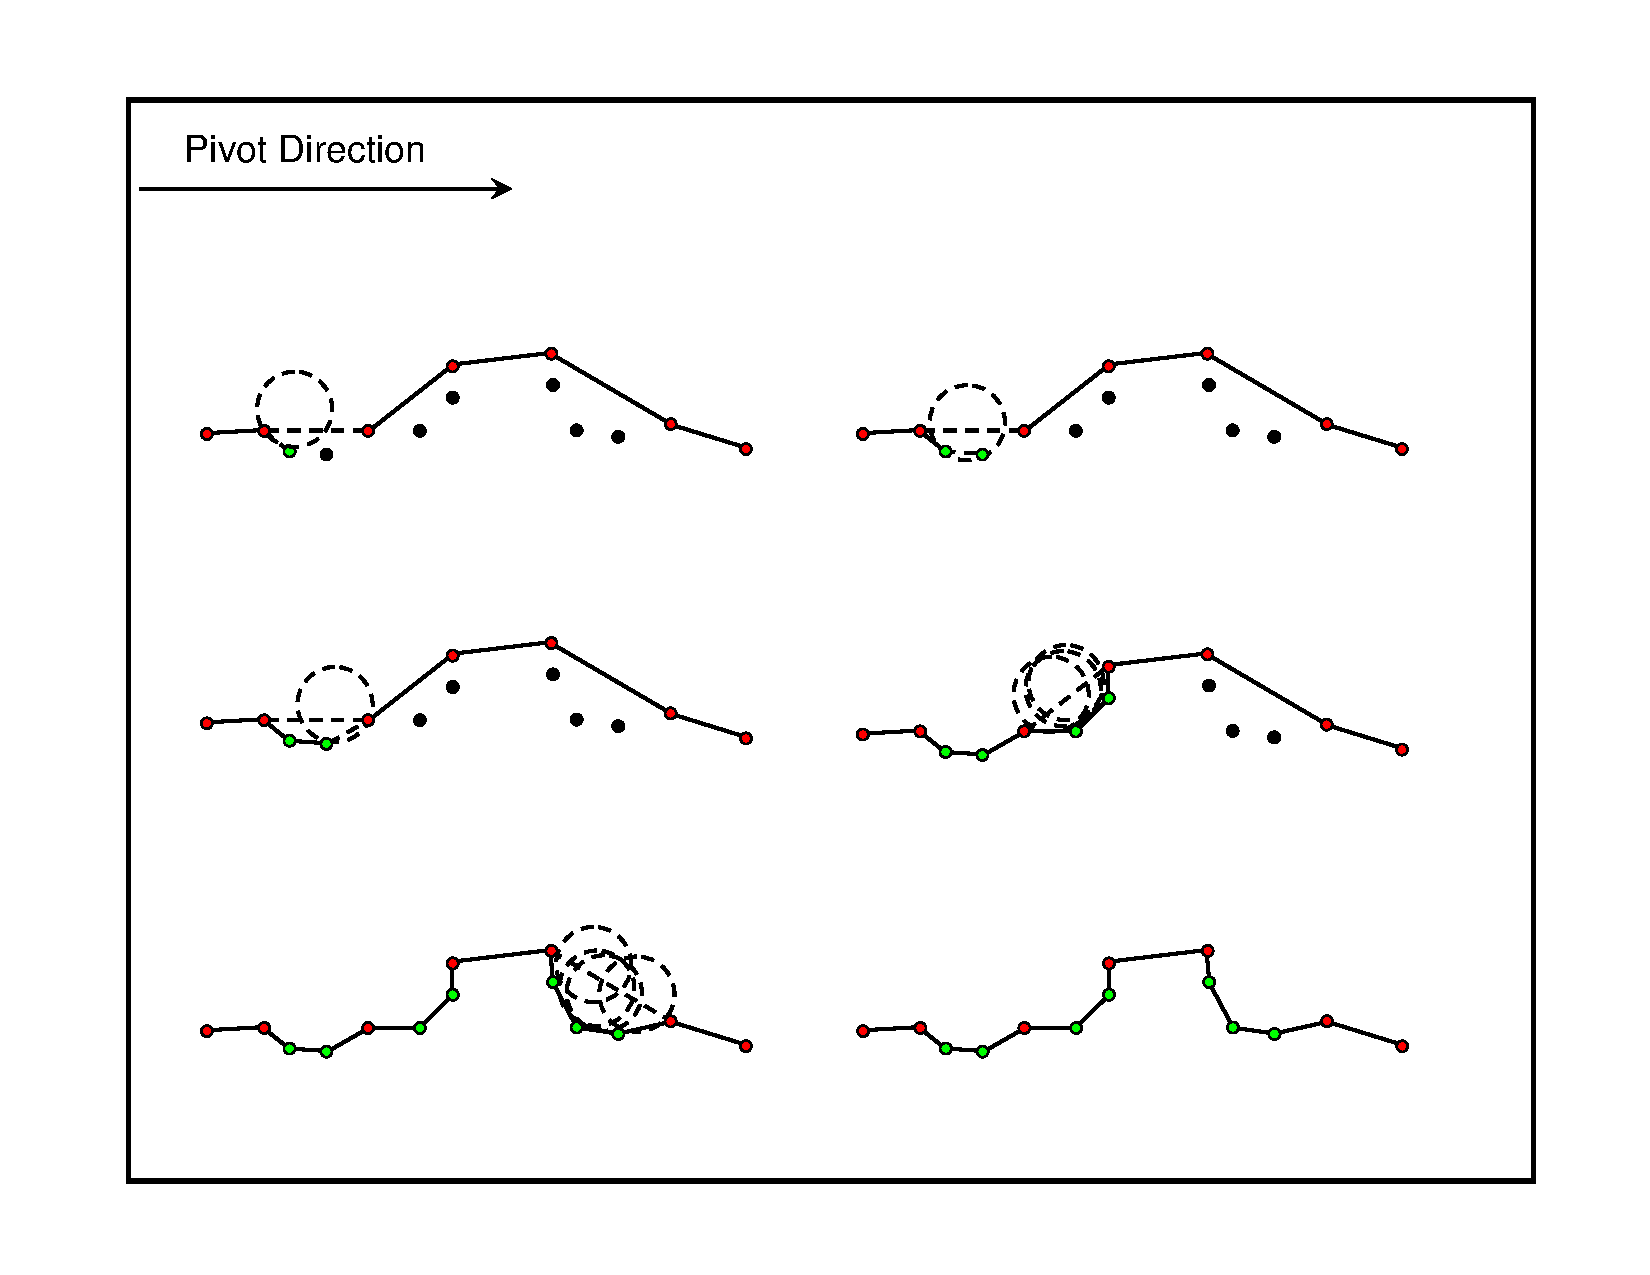
\includegraphics[width=0.8\textwidth]{BPA_refine.pdf} \\
(b)
\end{tabular}
\end{center}
\caption{Adaptive ball pivoting algorithm:
(a) Initial pivoting with a ball of radius 2$r$;
(b) Refinement with a ball of radius $r$.}
\label{fig:BPA}
\end{figure*}


The idea of the BPA is straight-forward:
pivot a ball on a starting point in the image
until it touches another data point as depicted in \Figa{BPA}.
Add the new touched
data point into an ordered list as the vertices of the contour polygon and
set it as the new pivoting point.
Keep doing this pivoting process until all data points are touched.

\section{Boundary Vectorization}
The basic idea behind the proposed framework for contour computation is as follows:
apply BPA on a selected starting point until
either the ball pivots back to the starting point which indicates a closed boundary is detected,
or the ball reaches a gap which means this contour is a non-closed
contour and one of the end points is reached.
Because the ball can start pivoting along either clock-wise direction or counter clock-wise direction,
another pivoting process at start pivoting from the other direction is conducted.
When both directions have been explored, a contour computation is done.
After this, the refinement process is carried out for each line segments using the same BPA algorithm.
For this refinement, the starting point is now the first end point of a line
and the stopping case is that the ball reaches the other point or it
reaches a gap.

Here is more detailed description for the algorithm.
At the initial BPA stage, a relatively large radius $r$ is chosen as a coarse step to cover all gaps between data points.
The output of the initial BPA, $\boldsymbol{\Phi}$, contains an ordered list of the boundary data
points $\boldsymbol{P}$ and their corresponding directions $\overrightarrow{\boldsymbol{R}}$ in which
the ball $C$ starts pivoting.
The BPA refinement process applies a smaller radius, say $r' = r/2$,
to $\boldsymbol{\Phi}$ to get more accurate results, as shown in \Figb{BPA}.
For this stage, the length of each line segment formed by adjacent points is checked,
$\ell = \overline{P_0P_1}$, in $\boldsymbol{\Phi}$.
For long line segments, the BPA is applied between the two adjacent points.
When the ball reaches the second end point, a new list of ordered boundary points,
$\boldsymbol{\Phi'}$, is inserted into $\boldsymbol{\Phi}$ between $P_0$ and
$P_1$.
This process continues until it finishes checking every adjacent point in $\boldsymbol{\Phi}$.
The refinement stops when $r'$ falls below threshold $\tau_r$.

The key parameter for the BPA algorithm to work successfully is finding
a good initial size of the ball for pivoting.
Here are some general guidances for choosing the radius. If a contour is known to be a closed polygon,
the initial radius should be big, e.g. the width of an image, to cover all gaps along the boundary.
Otherwise, if a boundary consists of sub-boundaries, one could select a relative small radius to start.

An example on the proposed framework is shown in \Fig{BPA_refinement}.
The initial BPA takes radius $\tau_r$ = 128,
which produced a coarse contour as shown in \Figa{BPA_refinement}.
\Figb{BPA_refinement} - \Figd{BPA_refinement} show that the contour is becoming more
accurate as the radius $\tau_r$ decreases from 32 to 2. Note that the original
image size is 1024x392 pixels as shown in \Figa{failed_case}.

\begin{figure}[htbp]
\begin{center}
\begin{tabular}{cc}
\fbox{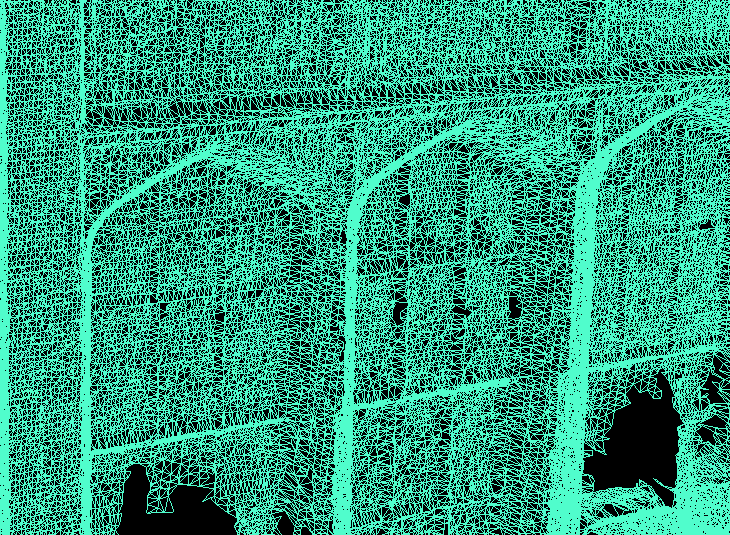
\includegraphics[width=0.45\textwidth]{BPA_TH.png}} &
\fbox{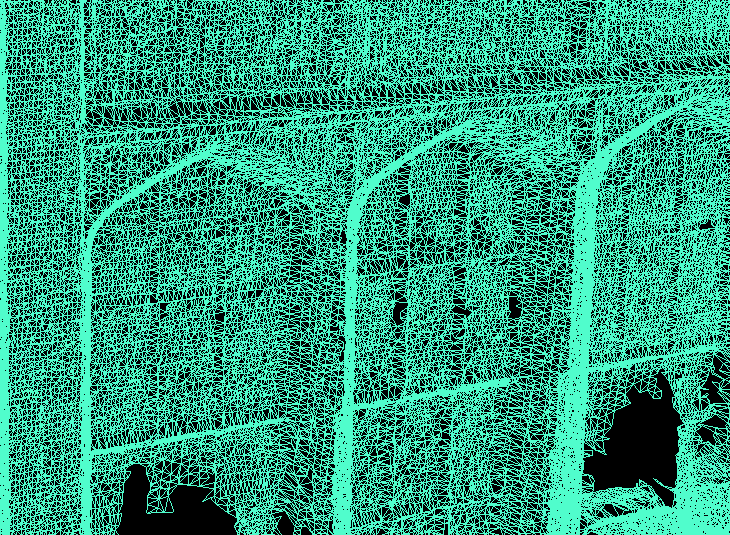
\includegraphics[width=0.45\textwidth]{BPA_TH.png}} \\
(a) & (b) \\
\fbox{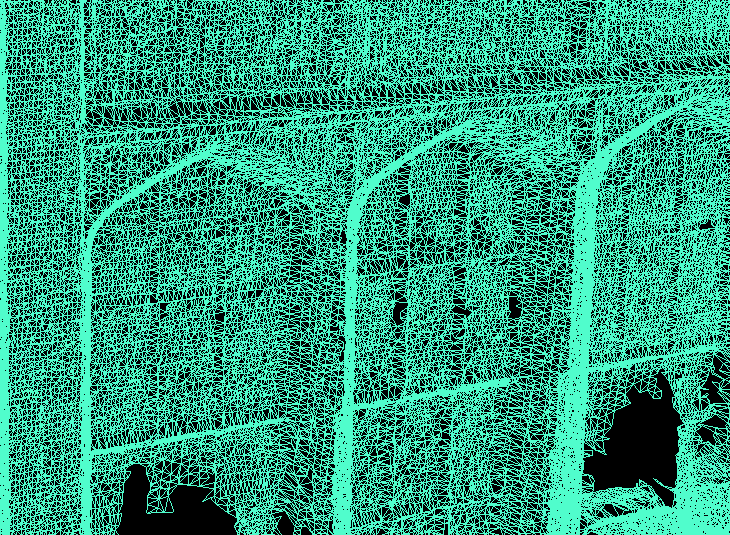
\includegraphics[width=0.45\textwidth]{BPA_TH.png}} &
\fbox{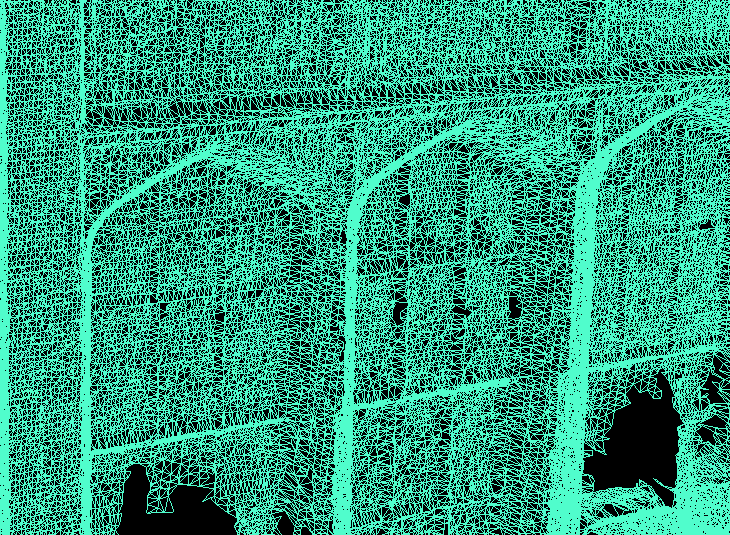
\includegraphics[width=0.45\textwidth]{BPA_TH.png}} \\
(c) & (d)
\end{tabular}
\end{center}
\caption{Boundary vectorization of a binary image with (a) radius = 128
(b) radius = 32 (c) radius = 8 (d) radius = 2.}
\label{fig:BPA_refinement}
\end{figure}


\begin{figure*}[htbp]
\begin{center}
\begin{tabular}{c}
\fbox{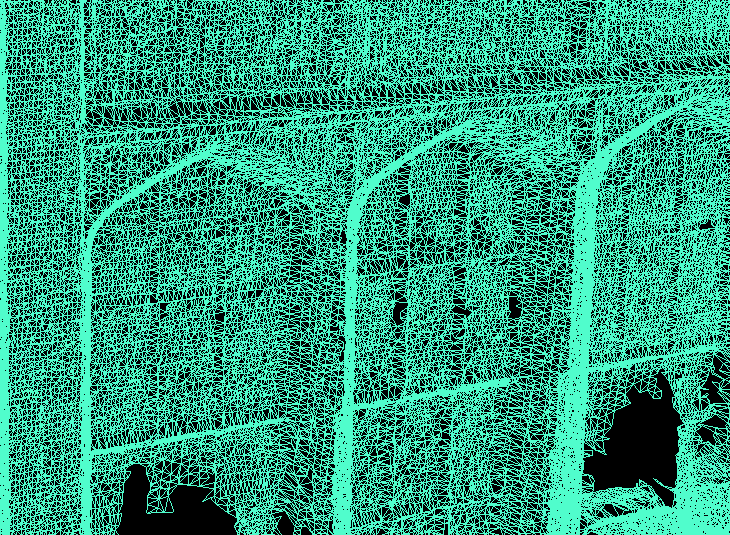
\includegraphics[width=0.7\textwidth]{BPA_TH.png}} \\
(a) \\
\fbox{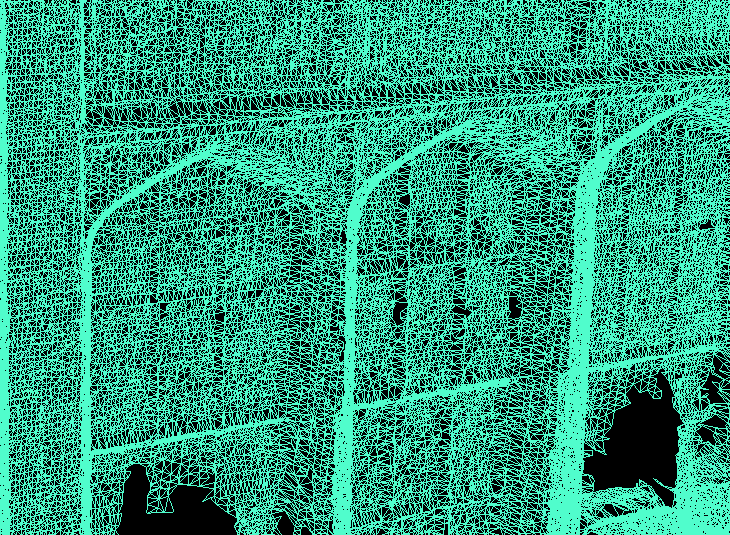
\includegraphics[width=0.7\textwidth]{BPA_TH.png}} \\
(b) \\
\fbox{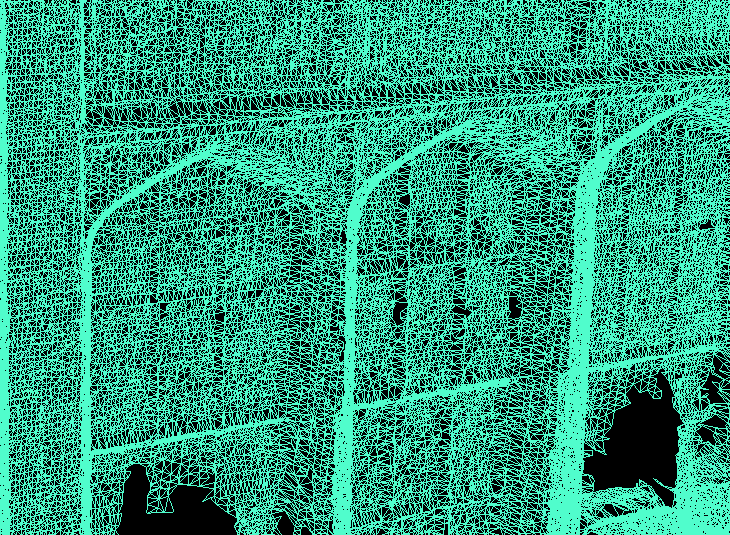
\includegraphics[width=0.7\textwidth]{BPA_TH.png}} \\
(c) 
\end{tabular}
\end{center}
\caption{(a) An example of binary image.
(b) The vectorization result based on DP algorithm and
(c) The vectorization result from proposed BPA algorithm.}
\label{fig:failed_case}
\end{figure*}

\begin{figure*}[htbp]
\begin{center}
\begin{tabular}{c}
\fbox{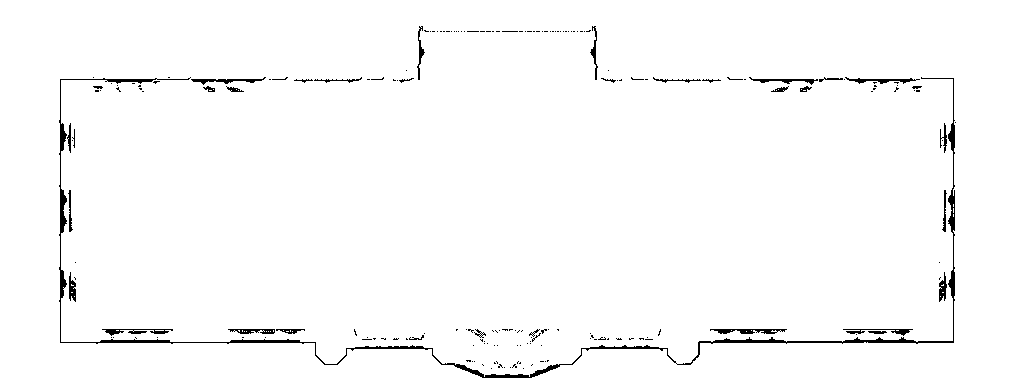
\includegraphics[width=0.7\textwidth]{aaa_image_slice_0529.png}} \\
(a) \\
\fbox{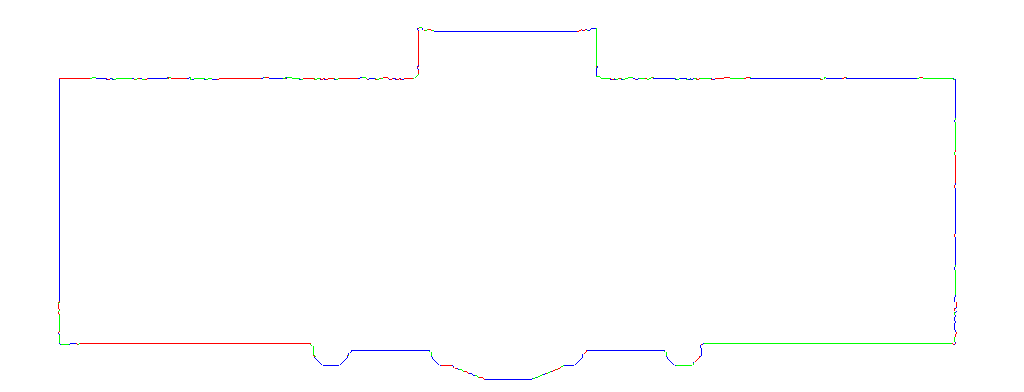
\includegraphics[width=0.7\textwidth]{bbb_image_slice_1024_392_0533_refine_with_rad_1_and_merged.png}} \\
(b) \\
\fbox{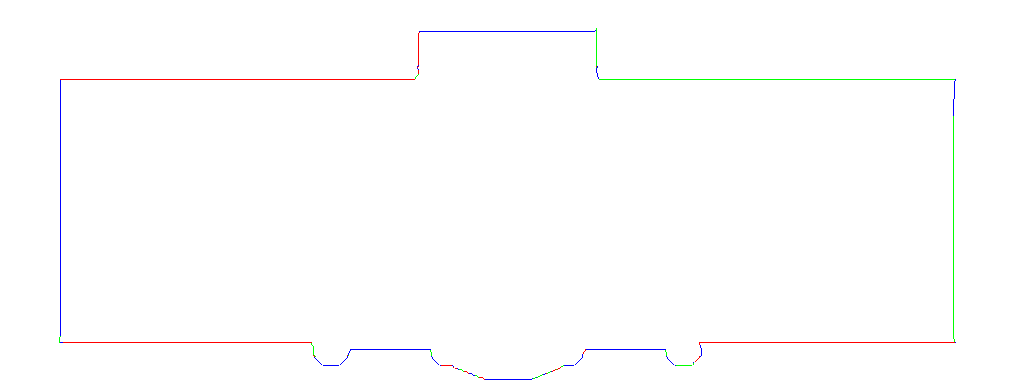
\includegraphics[width=0.7\textwidth]{bbb_image_slice_1024_392_0533_combine_HT_BPA_rad_32.png}} \\
(c)
\end{tabular}
\end{center}
\caption{Boundary vectorization of noisy binary image.
(a) the binary image to be processed.
(b) the contour computed by proposed method.
(c) the contour obtained by simplification with Hough transform.}
\label{fig:HT_BPA_figure}
\end{figure*}

\section{Contour Simplification}
\label{sec:BPA_HT}
%%% Adaptive BPA + HT %%%%

Although the proposed framework is an efficient and straightforward approach to
vectorize the contours of noisy images,
it might produce many short line segments for some special boundaries. An example
is shown in the upper part of the contour in \Figb{HT_BPA_figure} (Please see this
in zoomed-in mode). Here, each colored segment represents a contour edge.
One way to reduce the number of vertices of the polygon is to apply
the approximation polygon method in \cite{DP_AV}. The drawback of this
method is that the topological structures, such as straight lines, would be lost.
To solve this issue, a Hough transform (HT) based method is proposed to replace
short line segments with long lines and potentially eliminate noisy
or outlier vertices around the boundary.

To combine the adaptive BPA with HT, one can first apply the HT algorithm on the
original raster image $I$ to obtain all straight lines $\boldsymbol{L}$ and sort them by length.
The longer lines give higher confidence to the line structure of the underly images.
Then a dilation operation with 8-connected neighbors on $I$ can be used to get the dilation image, $I_d$.
The next step is to measure how well the lines in $\boldsymbol{L}$ match with
data in $I_d$, which determines whether a line in $\boldsymbol{L}$
should be used as a substitution or not.

If a line segment $L$ is found to be a good candidate, the next step is to
find the corresponding part of the BPA points in $\boldsymbol{\Phi}$ for
substitution. The first step is to compute the closest two points
$P_i$ and $P_j$ in $\boldsymbol{\Phi}$ to the two end points of $L$.
If the vertices in $\boldsymbol{\Phi}$ represent a polygon, they will have
a circle layout, i.e., $\boldsymbol{P} = \{ P_0,P_1,\ldots ,P_{n-1}, P_0 \}$.
Assuming $i < j$, there are two possible choices to replace
the series of the points, which are
$\boldsymbol{P_1} = \{ P_i,P_{i+1},\ldots,P_{j-1}, P_j \}$, and
$\boldsymbol{P_2} = \{ P_j,P_{j+1},\ldots,P_{i-1}, P_i \}$.
To determine which one is correct, one can compare the distance, $D$,
from the line $L$ to both set of the points $\boldsymbol{P_1}$ and
$\boldsymbol{P_2}$.
The point set with smaller $D$ is about to be substituted by the line $L$.
\begin{equation*}
D = \underset{\boldsymbol{P_1},\boldsymbol{P_2}}{\operatorname{arg\,min}}\sum{\lVert P_i - L \rVert}
\qquad P_i \in \boldsymbol{P_1} \ \text{or} \ P_i \in \boldsymbol{P_2}
\end{equation*}
where $\lVert P_i - L \rVert$ is the Euclidean distance from point $P_i$ to
line $L$.

After the integration of BPA contour with the Hough transform lines,
the beautified contour is shown in \Figc{HT_BPA_figure}.
Notice that the top part of the contour, which consisted of short line
segments, was replaced with two long line segments.
As one can see, this process reduces the noise, simplifies the contour, and produces clean results
for contours with straight line structures.

\begin{figure}[htbp]
\begin{center}
\begin{tabular}{ccc}
\fbox{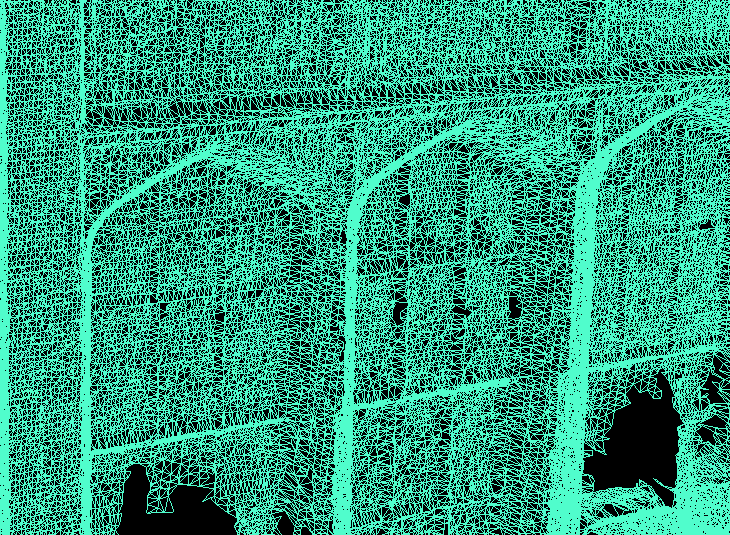
\includegraphics[width=0.3\textwidth]{BPA_TH.png}} &
\fbox{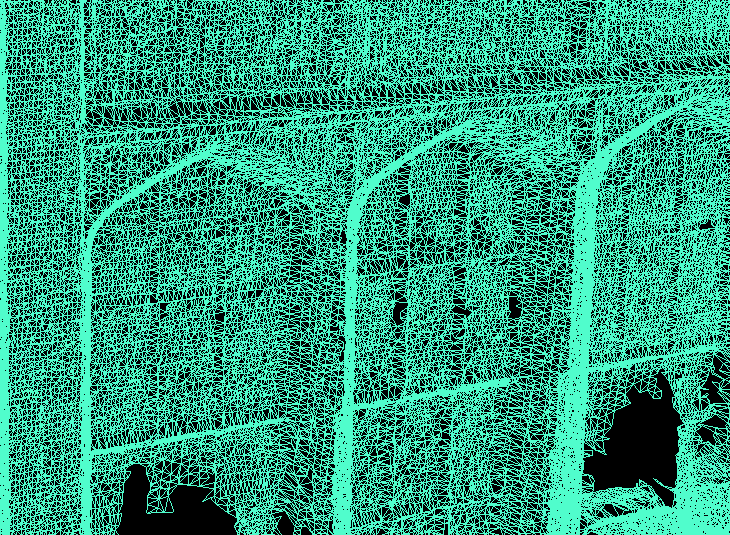
\includegraphics[width=0.3\textwidth]{BPA_TH.png}} &
\fbox{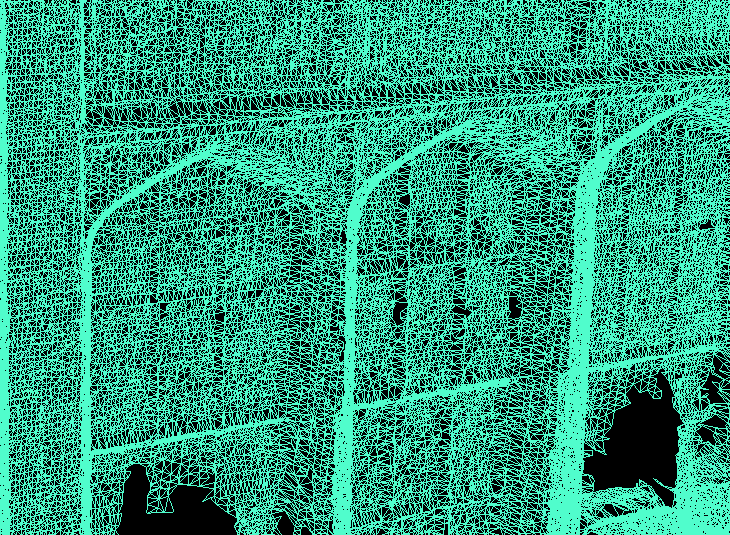
\includegraphics[width=0.3\textwidth]{BPA_TH.png}} \\
(a) & (b) & (c) \\
\fbox{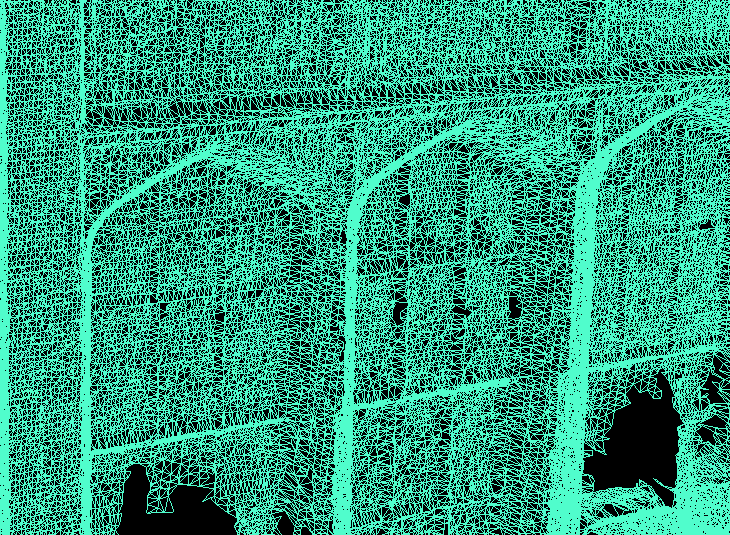
\includegraphics[width=0.3\textwidth]{BPA_TH.png}} &
\fbox{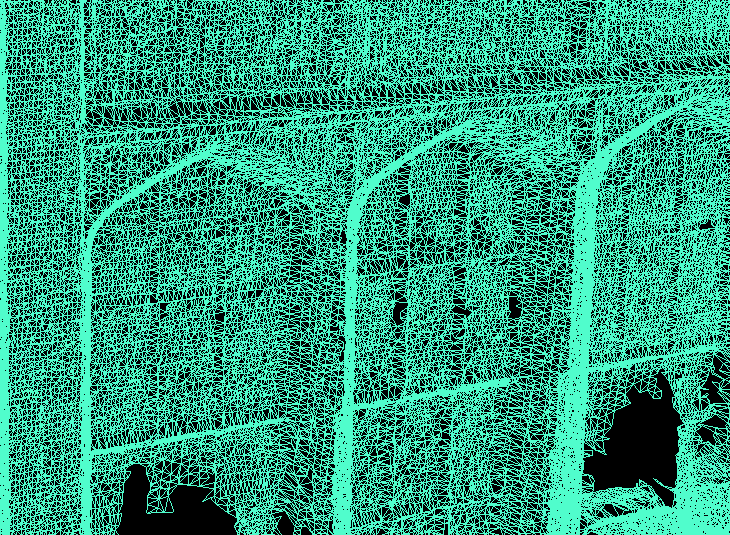
\includegraphics[width=0.3\textwidth]{BPA_TH.png}} &
\fbox{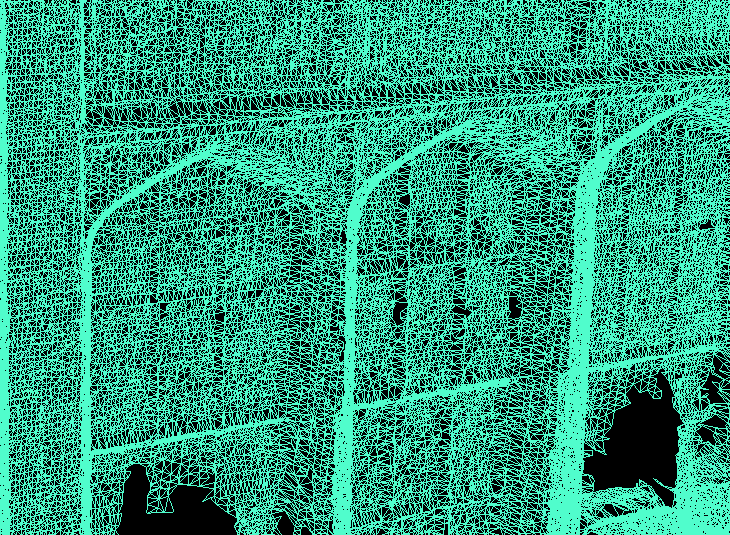
\includegraphics[width=0.3\textwidth]{BPA_TH.png}} \\
(d) & (e) & (f) \\
\fbox{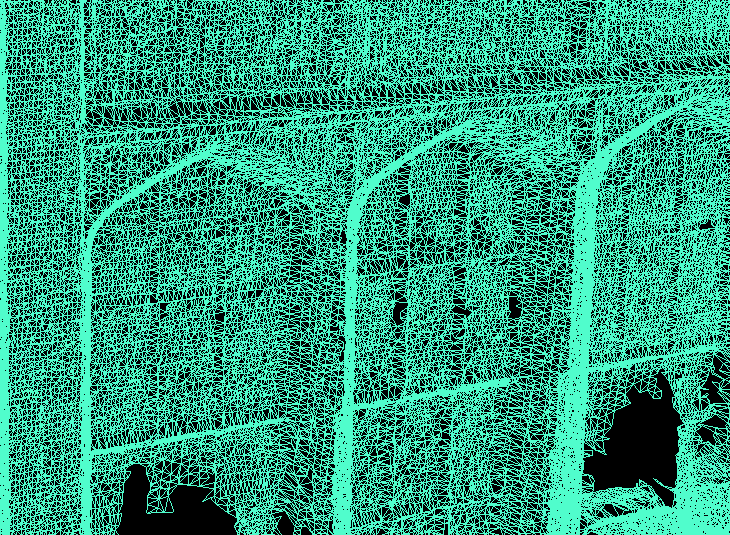
\includegraphics[width=0.3\textwidth]{BPA_TH.png}} &
\fbox{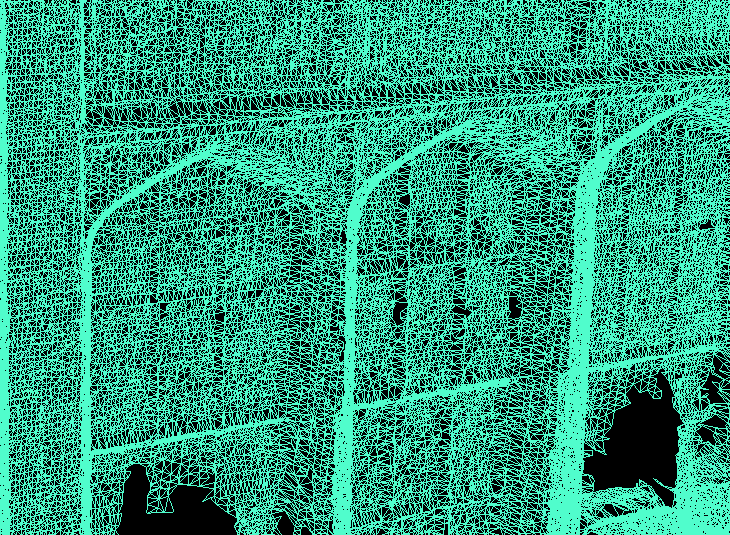
\includegraphics[width=0.3\textwidth]{BPA_TH.png}} &
\fbox{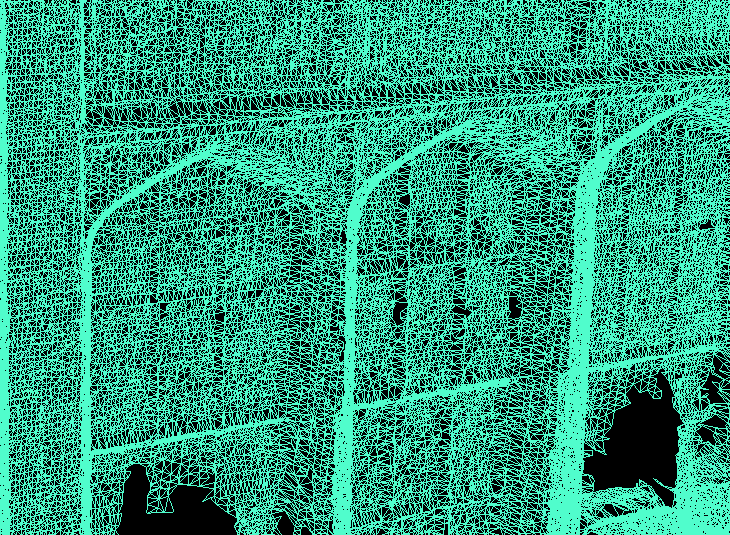
\includegraphics[width=0.3\textwidth]{BPA_TH.png}} \\
(g) & (h) & (i) \\
\end{tabular}
\end{center}
\caption{
More experimental results: (a), (d) and (g) show the original noisy binary images.
(b), (e) and (h) show the vectorization results from DP algorithm.
(c), (f) and (i) show the vectorization results from proposed algorithm.}
\label{fig:results}
\end{figure}

In addition to the results shown in \Fig{failed_case} and \Fig{HT_BPA_figure}, more
experimental results are shown in \Fig{results}. In the first row of \Fig{results},
the input image is of size 1024x392 and contains multiple contours.
In the second row, the input image is 800x640 and contains nested contours.
In the third row, the input image is 800x640 and contains a curved contour.
As one can see, the proposed framework can handle all the cases properly and fill the holes as expected, which
outperformed the standard DP algorithm.

%Several raster image vectorization approaches are proposed in
%\cite{DP_AAKMT,DP_DP}.
%The Douglas-Peucker algorithm attempts to connect all of the existing points
%to form a polygon.
%Although the implementation of this approach is very efficient with the
%improvement described in \cite{DP_HS}, this method cannot handle the case
%where spurious interior points are present, which contributes to outlier data.
%To tackle this issue, we adapted the ball-pivoting algorithm (BPA)
%\cite{BPA_BMRS} from its original use on 3D point cloud data to use on
%2D keyslice images where it produces vectorized boundaries.
%The key parameter for the BPA algorithm to work successfully is to
%find the right size of the ball for pivoting.
%We propose a coarse-to-fine adaptive BPA algorithm, described below,
%to solve this problem.
%
%\begin{figure}[hbtp]
%\centering
%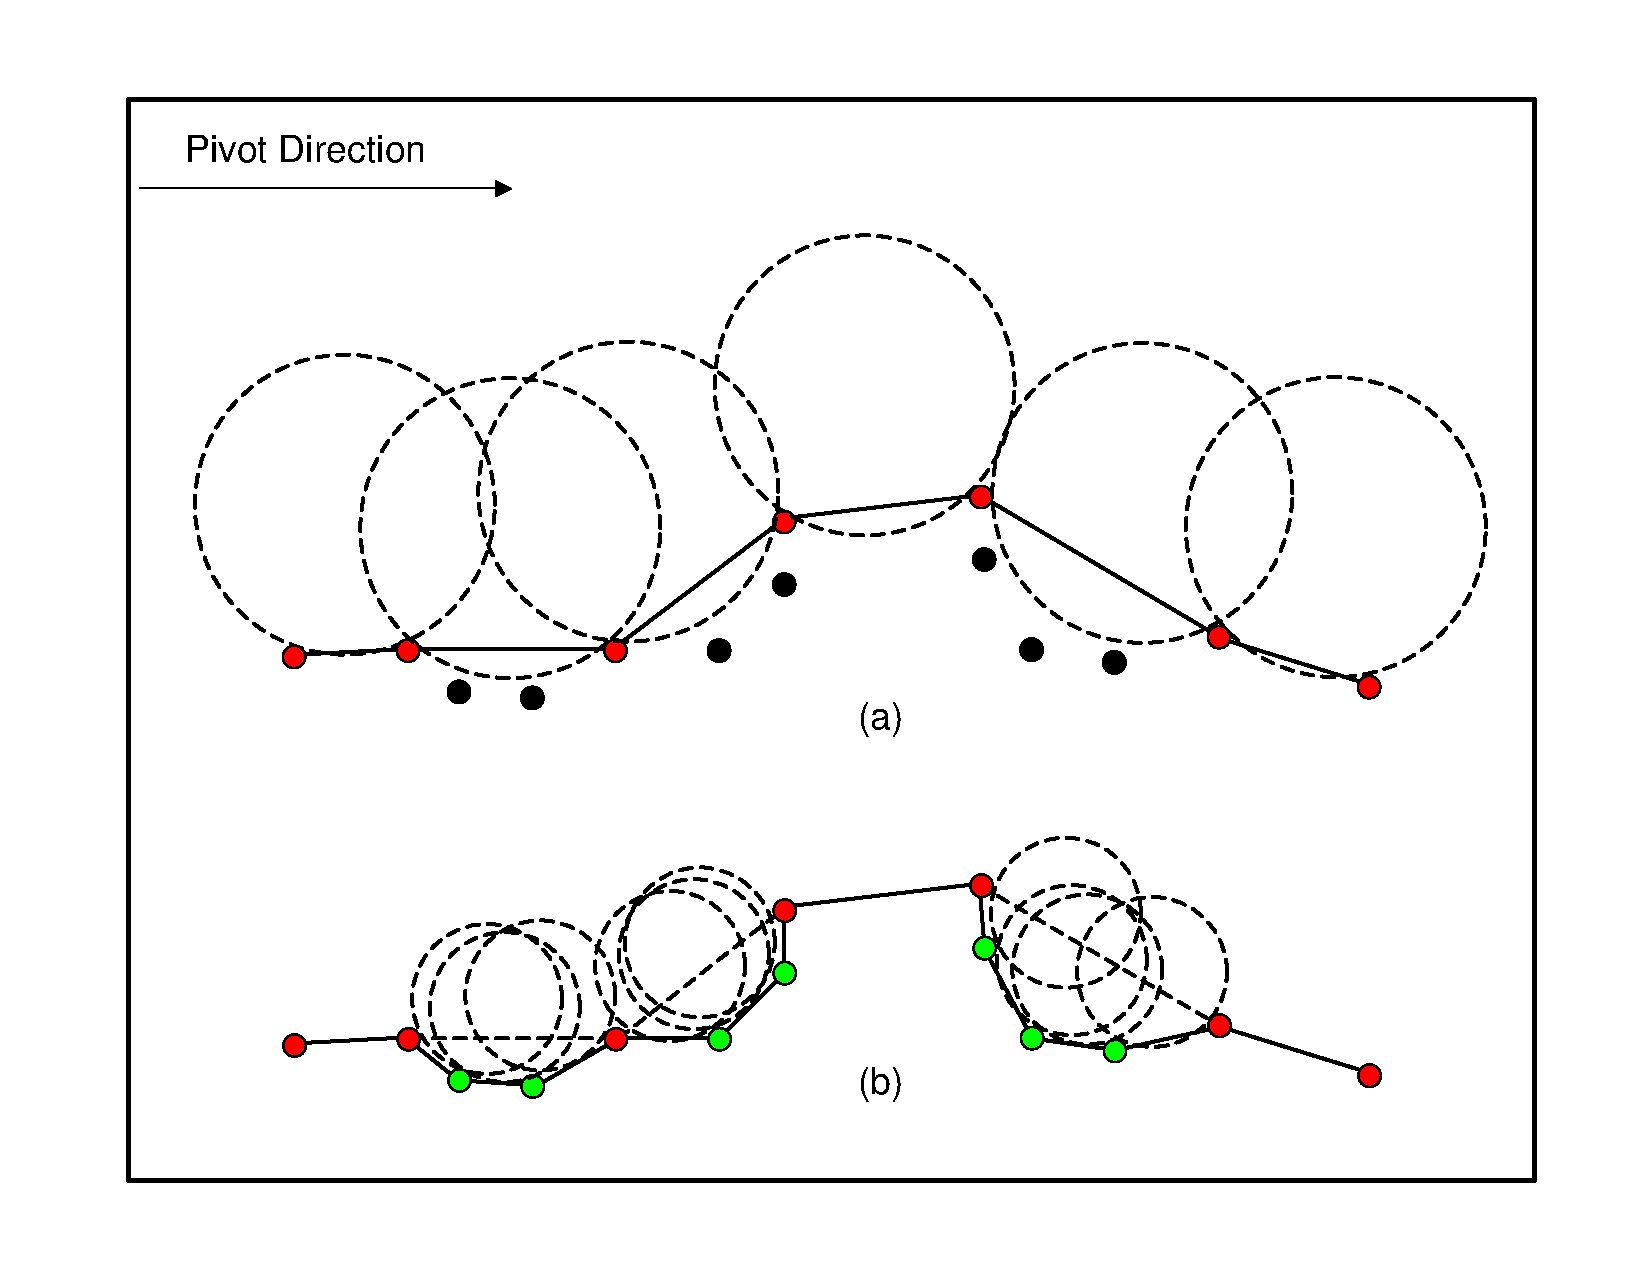
\includegraphics[width=0.8\textwidth]{figures/BPA.pdf}
%\caption{Adaptive ball pivoting algorithm:
%(a) Initial pivoting with circle of radius 2$r$;
%(b) Refinement with circle of radius $r$.}
%\label{fig:BPA}
%\end{figure}
%
%Due to the gap between data points, a relatively large radius $r$ is chosen
%as a coarse step to ensure that the ball will travel across all boundary
%data before turning back or reaching any existing boundary points.
%\Figa{BPA} shows an initial ball-pivoting process on 2D data points.
%The output of the initial BPA $\boldsymbol{\Phi}$ contains an ordered list of the boundary data
%points $\boldsymbol{P}$ and their corresponding directions $\overrightarrow{\boldsymbol{R}}$ in which
%the circle $C$ starts pivoting.
%The iterative BPA refinement process applies a smaller radius $r' = r/2$
%to $\boldsymbol{\Phi}$ to get more accurate results, as shown in \Figb{BPA}.
%The length of each line segment formed by adjacent points is checked,
%$\ell = \overline{P_0P_1}$, in $\boldsymbol{\Phi}$.
%If this line is long enough, the BPA is applied between the two adjacent points.
%When the ball reaches the second point, a new list of ordered boundary points,
%$\boldsymbol{\Phi'}$, is inserted into $\boldsymbol{\Phi}$ between $P_0$ and
%$P_1$.
%This process continues until it finishes checking every adjacent point in $\boldsymbol{\Phi}$.
%The refinement stops when $r'$ falls below threshold $\tau_r$.
%
%%%% Adaptive BPA + HT %%%%
%
%Although the adaptive BPA is a very efficient and straightforward approach to
%vectorize the contours of the building facade in the keyslice images,
%it produces many short line segments and is sensitive to noise, as shown
%in the upper part of the vectorized image in \Figa{HT_BPA_figure}.
%Based on the observation that the boundaries of man-made buildings are replete
%with lines, we can improve the adaptive BPA results by line fitting using the
%Hough transform (HT).
%
%\begin{figure}[htbp]
%\begin{center}
%\begin{tabular}{c}
%\fbox{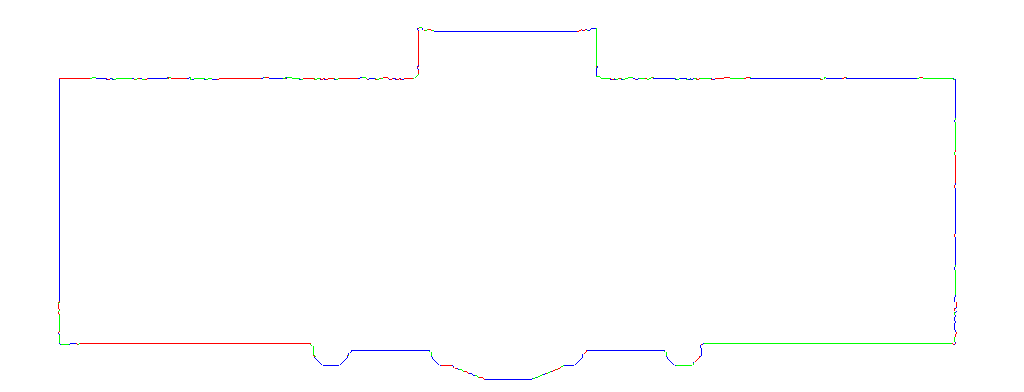
\includegraphics[width=0.6\textwidth]{bbb_image_slice_1024_392_0533_refine_with_rad_1_and_merged.png}} \\
%(a) \\
%\fbox{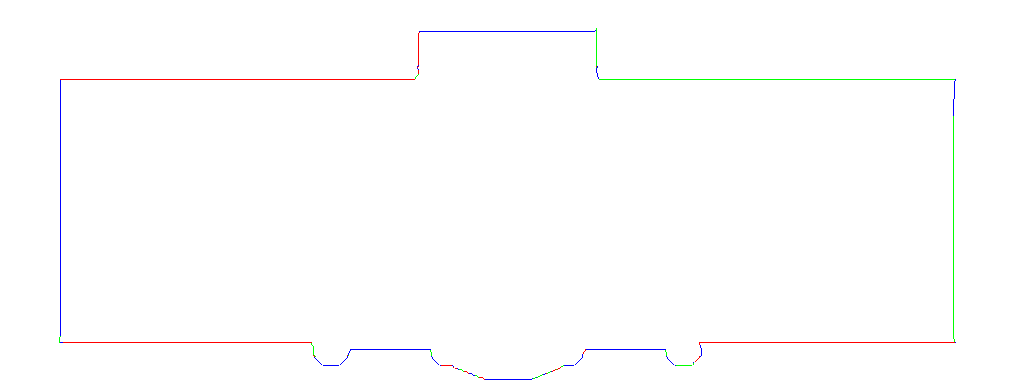
\includegraphics[width=0.6\textwidth]{bbb_image_slice_1024_392_0533_combine_HT_BPA_rad_32.png}} \\
%(b)
%\end{tabular}
%\end{center}
%\caption{Boundary vectorization of keyslice image with (a) adaptive BPA
%and (b) adaptive BPA / Hough transform.}
%\label{fig:HT_BPA_figure}
%\end{figure}
%
%To combine the adaptive BPA with HT, we first apply the HT algorithm on the
%keyslice image to obtain all lines $\boldsymbol{L}$ and sort them by length. 
%The longer lines give more confidence to the line structure of the building.
%We integrate the BPA and HT methods by first applying a dilation operation on
%$I$ using 8-connected neighbors to get the dilation image, $I_d$.
%The next step is to measure how well the lines in $\boldsymbol{L}$ match the
%data in $I_d$, which determines whether a line in $\boldsymbol{L}$
%should be used as a substitution or not.
%
%If a line segment $L$ is found to be a good candidate, the next step is to
%find the corresponding part of the BPA points in $\boldsymbol{\Phi}$ for
%substitution. To do this, we first compute the closest two points
%$P_i$ and $P_j$ in $\boldsymbol{\Phi}$ to the two end points of $L$.
%The points in $\boldsymbol{\Phi}$ represent a polygon and therefore form
%a circle layout, i.e., $\boldsymbol{P} = \{ P_0,P_1,\ldots ,P_{n-1}, P_0 \}$.
%Assuming $i < j$, there are two possible choices to replace
%the series of the points, which are
%$\boldsymbol{P_1} = \{ P_i,P_{i+1},\ldots,P_{j-1}, P_j \}$, and
%$\boldsymbol{P_2} = \{ P_j,P_{j+1},\ldots,P_{i-1}, P_i \}$.
%To determine which one is correct, one can compare the distance, $D$,
%from the line $L$ to both set of the points $\boldsymbol{P_1}$ and
%$\boldsymbol{P_2}$.
%The point set with smaller $D$ is about to be substituted by the line $L$.
%\begin{equation*}
%D = \underset{\boldsymbol{P_1},\boldsymbol{P_2}}{\operatorname{arg\,min}}\sum{\lVert P_i - L \rVert}
%\qquad P_i \in \boldsymbol{P_1} \ \text{or} \ P_i \in \boldsymbol{P_2}
%\end{equation*}
%where $\lVert P_i - L \rVert$ is the Euclidean distance from point $P_i$ to
%line $L$.
%
%After being replaced with line structures detected by the Hough transform,
%the beautified contour is shown in \Figb{HT_BPA_figure}.
%Notice that the top part of the contour, which consisted of short line
%segments, was refined with two long line segments.
%This reduces the noise, simplifies the contour, and produces clean models.
%
%

\begin{figure}[htbp]
\begin{center}
\begin{tabular}{c}
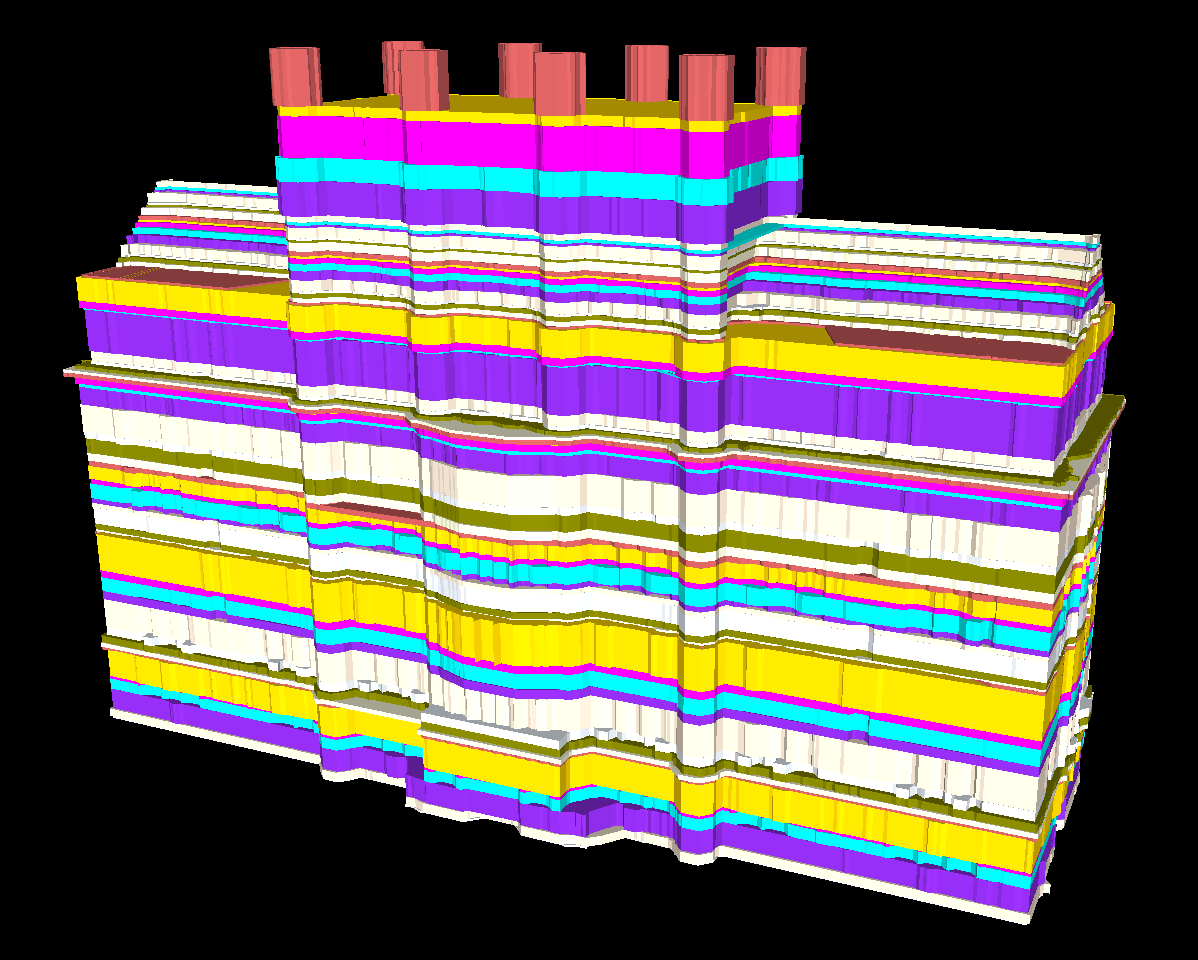
\includegraphics[width=0.8\textwidth]{notaper_8_4.png}
\end{tabular}
\end{center}
\caption{ The reconstructed model based on extrusion operation on keyslices. }
\label{fig:DXF_notaper_model}
\end{figure}

